\documentclass[runningheads]{llncs}
\usepackage{amsmath}
\usepackage{cite}
%
\usepackage[T1]{fontenc}
% T1 fonts will be used to generate the final print and online PDFs,
% so please use T1 fonts in your manuscript whenever possible.
% Other font encondings may result in incorrect characters.
%
\usepackage{graphicx}
% Used for displaying a sample figure. If possible, figure files should
% be included in EPS format.
%
% If you use the hyperref package, please uncomment the following two lines
% to display URLs in blue roman font according to Springer's eBook style:
%\usepackage{color}
%\renewcommand\UrlFont{\color{blue}\rmfamily}
%\urlstyle{rm}
%
\begin{document}
%
\title{FINDING NEMO: A Join-and-Evict Protocol for Bounded-Degree Random Overlay Construction}
%
\titlerunning{FINDING NEMO: Node Join-and-Evict Protocol}
% If the paper title is too long for the running head, you can set
% an abbreviated paper title here
%
\author{Ha Khai Nguyen\orcidID{0009-0009-8804-0042} \and
Huynh Phuc To \and
Duy Khanh Nguyen\orcidID{0009-0002-8639-4444} \and
Hoang Quan Ninh \and
Minh Duy Vo}
%
\authorrunning{H. K. Nguyen et al.}
% First names are abbreviated in the running head.
% If there are more than two authors, 'et al.' is used.
%
\institute{Vietnamese-German University, Ben Cat, Binh Duong, Vietnam
\url{https://vgu.edu.vn}}
%
\maketitle              % typeset the header of the contribution
%
\begin{abstract}
Decentralized overlay networks rely heavily on random regular topologies to guarantee critical properties such as low diameter and resilience to massive node failures. 
While existing literature extensively analyzes macroscopic outcomes like network expansion and churn tolerance, it frequently overlooks the micro-level mechanics of node integration. 
Specifically, achieving join-specific bounded-degree randomness remains an open challenge: how can a single joining node reach a fixed target degree through local edge redistribution without injecting structural biases into the network's indegree, clustering, and load?

To address this gap, we present FINDING NEMO, a novel, fully decentralized join-and-evict protocol tailored explicitly for bounded-degree random overlay construction. 
During the joining phase, a new node samples existing network members to fulfill its target connection count. 
To strictly maintain the bounded degree constraint, fully connected target nodes accommodate the joining node by evicting an existing neighbor; this evicted neighbor is subsequently rewired to connect directly with the new node.

This localized, structured neighbor discovery mechanism ensures that the joining node seamlessly reaches its fixed degree. More importantly, it dynamically distributes connections while rigorously preserving the bounded network density and uniform structural randomness of the overlay. 
By isolating these exact micro-level join rules, our work demonstrates that eviction-triggered rewiring successfully sustains a structurally unbiased topology, providing a resilient and balanced foundation for dynamic peer-to-peer systems.

\keywords{Distributed Systems \and Peer-to-Peer \and Node Joining.}
\end{abstract}
%
%
%

\section{Introduction}
In distributed systems, network formation plays an important role in coordination between nodes. 
For example, it is crucial that nodes are connected to each other in a way that allows their health state to be effectively checked and acknowledged by others within a peer-to-peer (P2P) overlay \cite{dadgarLifeguardLocalHealth2017,yangMedleyMembershipService2022}. 
One highly effective method for achieving this is to construct a random regular graph, which inherently ensures that the system remains highly scalable \cite{lawDistributedConstructionRandom2003,guptaFullyDistributedProtocolConstructing2025,CYCLONInexpensiveMembership,poonpakdeeRobustEfficientMembership2017}.

However, while research on the low diameter, peer sampling, and expander maintenance of these topologies has been extensively conducted \cite{lawDistributedConstructionRandom2003,guptaFullyDistributedProtocolConstructing2025,CYCLONInexpensiveMembership,poonpakdeeRobustEfficientMembership2017}, only a limited amount of work has focused on the specific join rules required to ensure unbiased bounded-degree randomness. 
The literature is rich on whole-overlay outcomes, but thin on micro-level join rules—such as eviction-triggered rewiring—and the structural biases they can introduce. 

To address this exact problem, we propose our algorithm, FINDING NEMO, which stands for Finding Neighbors and Evicting Members of their Own. 
By isolating the neighbor discovery protocol, we mathematically and empirically demonstrate how a single node can integrate into an overlay while preserving its strictly regular topology.

\section{Preliminaries and Network Model}
In our network model, we operate under the foundational assumption that each node must attempt to maintain a fixed $k$ number of neighbors. 
This constraint ensures that the overlay is neither too dense (which would negatively affect the scalability and bandwidth of the system) nor too scarce (which would risk node isolation and fragmentation). 
This requirement is derived from our previous work in decentralized node health checking, where each node must be supervised by a sufficient, strictly bounded number of peers to eliminate false-positive failure detections. 
Furthermore, the target degree $k$ must be an even integer, a property that is mathematically necessary for our edge-rewiring methodology.

Regarding operational complexity, it takes $n$ messages for a newly spawned node to broadcast its initial join request to an $n$-node network. 
In response, the requested nodes communicate with one of their existing neighbors under specific conditions to execute edge hand-offs. 
However, because $k$ is a strict constant, these local edge-rewiring behaviors do not grow exponentially as the network expands, ensuring asymptotic efficiency.

\section{The FINDING NEMO Protocol}
To facilitate a rigorous understanding of the algorithm, several foundational terms and system rules are first defined:

\begin{itemize}
    \item \textbf{Neighbor:} A bidirectional relationship established between two nodes in the network. 
    If node A is a neighbor of node B, then node B is strictly considered a neighbor of node A.
    \item \textbf{Neighbor List:} A local data structure maintained independently by each node that stores information about its neighbors, such as their network addresses. 
    The neighbor list has a fixed capacity of $k$, where $k$ is an even number. 
    To maintain network connectivity and resilience, each node continuously attempts to keep its neighbor list as full as possible whenever sufficient peers are available.
\end{itemize}

The FINDING NEMO protocol begins when a newly created node requests to join the network. 
To promote random neighbor selection, the joining node broadcasts a join request to all existing nodes. 
Assuming ideal network connectivity, two primary topological cases are considered:

\subsubsection{Case 1: Small Network Phase.} 
If the network contains at most $k+1$ nodes, the joining node establishes connections with all existing nodes. 
This allows the node to reach its desired neighbor count without requiring any complex restructuring or eviction within the existing network topology. 
For example, in a network consisting of four nodes with a target neighbor count of $k=4$, a fifth joining node simply establishes connections with all four existing nodes, thereby satisfying its neighbor requirement directly.

\subsubsection{Case 2: Scaled Network Phase.} 
If the network contains more than $k+1$ nodes, it is mathematically assumed that all existing nodes have already reached their target neighbor count of $k$. 
Nevertheless, these fully connected nodes still acknowledge the new join request. 
After collecting all acknowledgements, the joining node constructs a \textit{join plan} by randomly selecting exactly $k/2$ responding nodes. 

The joining node immediately establishes initial connections with these selected nodes. 
Subsequently, each selected target node is instructed to randomly evict one of its current neighbors. 
These evicted nodes are then instructed to establish connections with the joining node. 
Consequently, the joining node acquires $k/2$ neighbors directly from the selected targets and an additional $k/2$ neighbors from the evicted nodes, resulting in a perfectly balanced total of $k$ neighbors. 

This process successfully maintains bounded network density while preserving uniform randomness in neighbor assignment, thereby reducing the likelihood of structural bias within the topology. 
In practice, a hybrid selection strategy is employed where nodes whose neighbor lists are not yet full are prioritized during the acknowledgement phase, accelerating the completion of underpopulated lists.

\section{Structural and Theoretical Guarantees}
A critical design question arises when scaling the network: why utilize a complex join-and-evict strategy rather than a simple join-only mechanism? 
This question strictly applies to the scaled network case, where all existing nodes are already equipped with a full neighbor list. 

By the Handshake Lemma, the total number of connections (edges) in a $k$-regular graph of $n$ nodes is exactly $nk/2$. 
If a single new node joins and the regular property is to be preserved, the total number of edges must grow to $(n+1)k/2$. 
The mathematical difference in required edges before and after the join is exactly $k/2$. 
If the new node simply creates $k$ new connections without triggering any evictions, the defined bounded-degree graph structure is destroyed. 
Therefore, to guarantee topological preservation, the protocol must break exactly $k/2$ existing connections and rewire them, which forms the exact mathematical foundation of FINDING NEMO.

\subsection{Guarantee of Graph Simplicity}
In theoretical random regular graph generation, uniform pairings frequently result in invalid topologies containing self-loops or multi-edges. 
Under the Configuration Model, the expected number of self-loops in a random pairing follows a Poisson distribution with a mean of $\lambda_1 = \frac{k-1}{2}$. 
Similarly, the expected number of multi-edges follows a mean of $\lambda_2 = \frac{(k-1)^2}{4}$. 
Consequently, the probability of naturally forming a simple graph—free of these structural defects—decays asymptotically as $\exp\left(-\frac{k^2 - 1}{4}\right)$. 

FINDING NEMO theoretically bypasses this probabilistic decay. 
By programmatically tracking an exclusion set during the join plan construction to strictly filter out the joining node's own identifier and previously selected targets, the protocol deterministically guarantees a simple graph topology with zero self-loops and zero multi-edges.

\subsection{Asymptotic Uniformity and Bias Resistance}
To preserve structural robustness, the network must avoid topological biases such as preferential attachment, which naturally creates disproportionately dense hubs. 
In the theoretical Configuration Model, unbiased random graphs are constructed by uniformly matching $nk$ total half-edges. 

FINDING NEMO effectively simulates this mathematically unbiased process in a decentralized environment. 
By enforcing uniform random sampling of existing targets, followed by the uniform random selection of an eviction victim from the target's existing neighbor list, the protocol perfectly mimics the breaking and re-pairing of a random half-edge. 
This guarantees that the localized join-and-evict logic actively resists structural bias, strictly preserving the bounded network density and uniform randomness required for high fault tolerance.

\subsection{Formal Space Complexity Bounds}
Formalizing the memory footprint of the algorithm provides a hard mathematical guarantee of its horizontal scalability. 
\begin{itemize}
    \item \textbf{Steady-State Complexity:} Because each node is strictly bounded to a predefined, even integer $k$, the permanent local routing table requires only $O(k)$ space. Relative to the total network size $n$, this guarantees an $O(1)$ permanent storage footprint per node. This ensures the protocol remains viable for memory-constrained devices even as the network scales to millions of nodes.
    \item \textbf{Transient Complexity:} During the initial broadcast phase, the joining node must temporarily buffer acknowledgements from the active network to construct its join plan. This necessitates an $O(n)$ space allocation. However, this memory spike is strictly limited to the brief vulnerability window prior to the execution of the final join plan.
\end{itemize}

\subsection{Resistance to Topological Fragmentation}
To evaluate the protocol's structural robustness, we analyze a theoretical null model: the probability that a simultaneous burst of $2k+2$ nodes joining an empty space results in a partitioned network consisting of two disconnected cliques of size $k+1$. Using the Bender-Canfield Configuration Model, we know the vast majority of random pairings naturally result in a globally connected uniform graph. 

However, under the specific mechanics of FINDING NEMO, nodes form via sequential or concurrent broadcasts rather than uniform static sampling. For a perfect topological split to occur, every node in Group A must completely fail to receive the initial broadcast messages from every node in Group B, and vice versa. Let $p$ be the probability of an unseen broadcast message due to network loss. The probability of this catastrophic splitting occurring during FINDING NEMO is given by:

$$P(\text{split}) = p^{2(k+1)^2}$$

Because this probability decays exponentially as the degree $k$ increases, we mathematically prove that our network design is highly resistant to splitting or fragmentation, requiring a near-total collapse of cross-group communication to partition.

\section{Concurrency and Vulnerability Modeling}
While FINDING NEMO provides strong guarantees for bounded-degree randomness, its purely decentralized nature introduces a vulnerability during massive concurrent network churn. 
When multiple nodes join simultaneously, they independently create join plans. 
If these plans contain duplicate target nodes, a concurrent bootstrap race occurs. 
Because a target node has a strict degree limit, conflicting requests are denied, leaving the rejected joining nodes deficient (under-connected).

We formalize this concurrency conflict using a thinned Poisson arrival process. 
Let $\lambda$ be the global arrival rate of new nodes (joins per second), $\tau$ be the network vulnerability window (delay from broadcast to execution), and $n$ be the existing network size. 
During a scaled join, a new node randomly selects $k/2$ targets from the $n$ available members. 

The arrival of join requests at a specific target node $A$ occurs at a localized rate of $\lambda_A = \lambda \frac{k}{2n}$. 
The number of requests, $X$, that arrive at node $A$ during the vulnerability window $\tau$ follows the Poisson distribution:

$$P(X = x) = \frac{(\lambda_A \tau)^x e^{-\lambda_A \tau}}{x!}$$

A collision occurs if Node $A$ receives two or more requests ($X \ge 2$) during $\tau$. 
This formally proves that as the global churn rate $\lambda$ increases, the probability of concurrent rejections grows exponentially. 
This mathematical limitation establishes the baseline necessity for future self-healing rewiring mechanisms.

\section{Simulation Results}
\label{sec:simulation_results}
To empirically validate the structural invariants, scalability, and concurrency boundaries of the FINDING NEMO protocol, an extensive discrete-event simulation framework was developed. 
The simulation suite isolates the neighbor discovery and join-and-evict mechanisms, evaluating topology formation across three distinct operational regimes: initial bootstrap convergence, horizontal scalability under long sequences of churn, and vulnerability to simultaneous concurrent joins. 
In total, more than 2,700 independent simulation runs were executed across varied parameter spaces.

\subsection{Experimental Setup and Evaluation Criteria}
\label{subsec:sim_setup}
The simulator models an overlay where peer communication is message-driven and asynchronous. 
Each joining node broadcasts an integration request, collects acknowledgements from existing members, formulates a deterministic join plan, and executes localized edge hand-offs. 
Network latency is modeled as an independent stochastic delay bounded by a vulnerability window $\tau$.

Following the formal verification criteria of decentralized overlay maintenance, we establish the following state definitions to classify topology health at each simulation phase:
\begin{itemize}
    \item \textbf{Non-mutual Edge:} A directional mismatch where node $u$ lists $v$ as a neighbor but $u \notin N_v$ (or vice versa). Because our overlay model mandates bidirectional supervision, any asymmetry constitutes a corrupted link.
    \item \textbf{Problematic Node:} An active node $u$ that violates at least one topological invariant: $\deg(u) \neq k$, self-referential links ($u \in N_u$), duplicate cache entries, or non-mutual relationships.
    \item \textbf{Network Convergence:} A terminal state where the overlay forms a single connected component with zero problematic nodes, verifying that every node satisfies exact $k$-regularity with valid, mutual edges.
\end{itemize}
The primary evaluation metric is the \textit{Convergence Success Rate} (\%), defined as the proportion of independent trials that attain valid network convergence without leaving deficient or disconnected nodes.

\subsection{Test 1: Bootstrap Convergence in Sparse Networks}
\label{subsec:test1_bootstrap}
Test 1 evaluates the bootstrap phase corresponding to Case~1 (Small Network Phase), where $k+1$ nodes are deployed into an empty network simultaneously. 
We varied the target degree limit across all even integers $k \in \{2, 4, 6, \dots, 20\}$, executing 50 independent trials for each degree (500 total runs).

\begin{figure}[t]
\centering
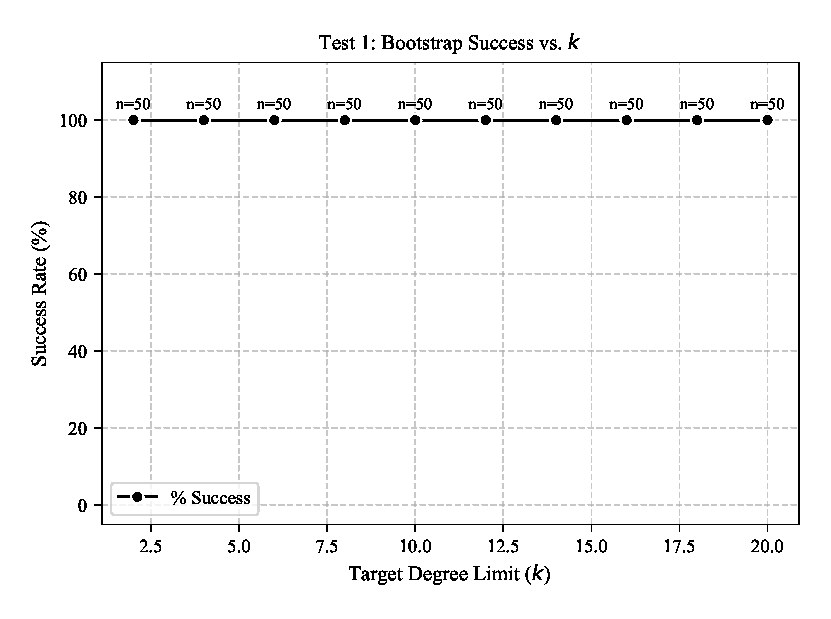
\includegraphics[width=0.60\textwidth]{eval_fig/test1_bootstrap.eps}
\caption{Test 1: Bootstrap success rate as a function of target degree limit $k \in [2, 20]$ in an empty network of $n = k+1$ nodes (50 independent trials per configuration, 500 total runs).}
\label{fig:test1_bootstrap}
\end{figure}

As shown in Fig.~\ref{fig:test1_bootstrap}, FINDING NEMO achieves a 100\% convergence success rate across every evaluated degree limit $k \in [2, 20]$. 
During this initial deployment phase, the total node count $n$ does not exceed $k+1$. 
Consequently, newly arrived nodes directly connect to all active members without executing edge evictions, forming a complete graph $K_{k+1}$ in which every node trivially satisfies $\deg(u) = k$. 
These results empirically confirm that the protocol's small network bootstrapping logic is unconditionally stable and free of structural deadlocks regardless of degree scale.

\subsection{Test 2: Scalability under Sequential Churn}
\label{subsec:test2_churn}
Test 2 evaluates the protocol's ability to scale dynamically under prolonged sequential churn, corresponding to Case~2 (Scaled Network Phase). 
Beginning with an established, converged network of $k+1$ nodes, new nodes are injected sequentially one by one up to $g$ total additions, where $g \in \{5, 10, 20, 30, 40, 50, 75, 100\}$. 
We systematically swept target degree limits $k \in \{4, 6, 8, 10\}$, executing 20 trials for each $(k, g)$ pair (640 total simulation runs).

\begin{figure}[t]
\centering
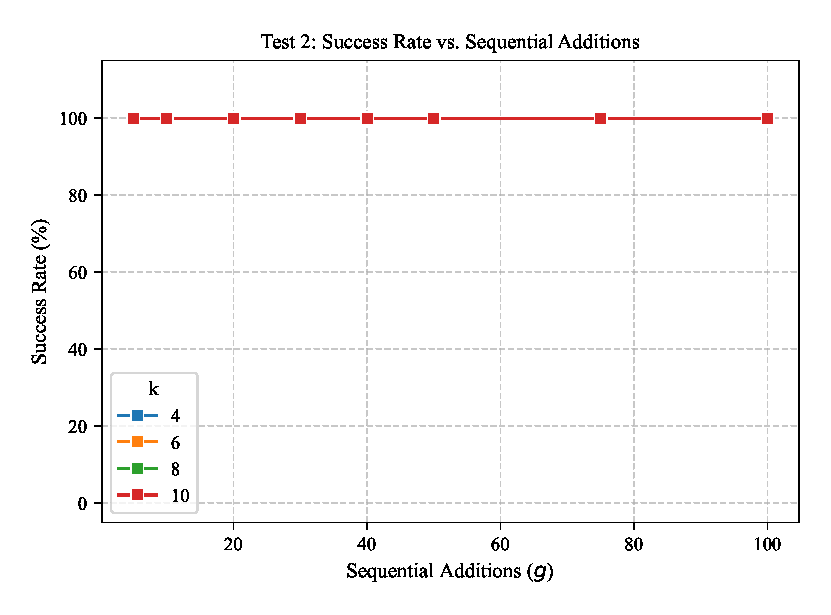
\includegraphics[width=0.49\textwidth]{eval_fig/test2_success_vs_g.eps}\hfill
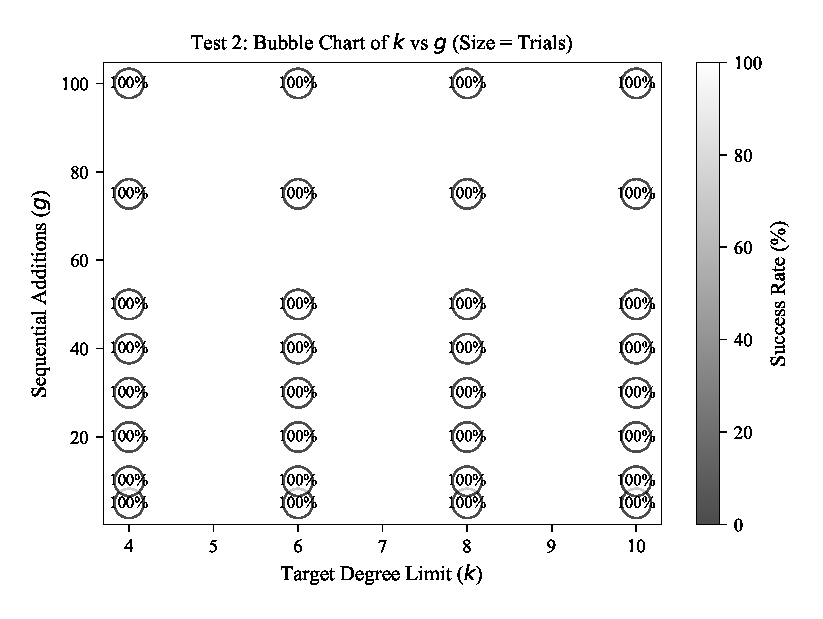
\includegraphics[width=0.49\textwidth]{eval_fig/test2_bubble_k_vs_g.eps}
\caption{Test 2 (Scalability under Sequential Churn): (a) Convergence success rate as a function of sequential additions $g \in [5, 100]$ for degrees $k \in \{4, 6, 8, 10\}$; (b) Complete parameter sweep bubble chart mapping $k$ versus $g$, where circle area is proportional to the number of trials (20 trials per configuration, 640 total runs).}
\label{fig:test2_results}
\end{figure}

Figure~\ref{fig:test2_results}(a) plots the success rate as a function of sequential additions $g$, while Fig.~\ref{fig:test2_results}(b) presents the complete parameter sweep bubble chart. 
Remarkably, FINDING NEMO sustained a 100\% convergence success rate across all 32 configuration pairs. 
Even after $g = 100$ sequential join operations (expanding the overlay to $100 + k + 1$ nodes), zero problematic nodes or partitioned clusters emerged. 
Each sequential join accurately identified $k/2$ fully-connected target peers, induced uniform edge evictions, and rewired the displaced endpoints to the joining node. 
This provides empirical validation of the Handshake Lemma conservation principle ($\Delta E = k/2$) established in Section~4, proving that sequential eviction hand-offs preserve exact $k$-regularity and global connectivity indefinitely without degree drift.

\subsection{Test 3: Concurrency Boundaries and Poisson Collision Modeling}
\label{subsec:test3_burst}
While sequential joins exhibit deterministic stability, simultaneous node arrivals introduce target contention during the vulnerability window $\tau$. 
Test 3 stress-tests this boundary by injecting a concurrent burst of $s$ nodes simultaneously into an established $k+1$ network, where $s \in \{1, 2, 3, 4, 5, 6, 8, 10, 12, 15, 20, 25, 30\}$. 
We evaluated degrees $k \in \{4, 6, 8, 10\}$ across 30 independent trials per configuration (1,560 total runs).

\begin{figure}[t]
\centering
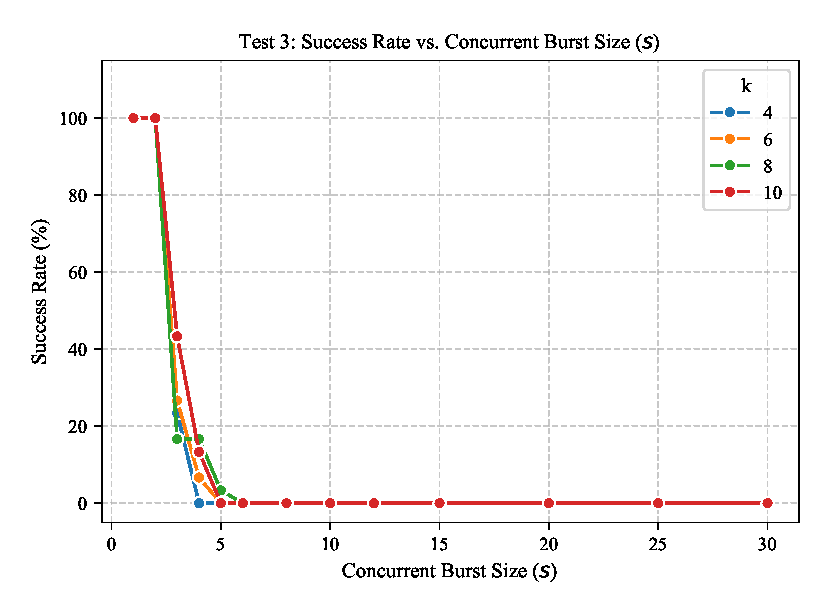
\includegraphics[width=0.49\textwidth]{eval_fig/test3_success_vs_s.eps}\hfill
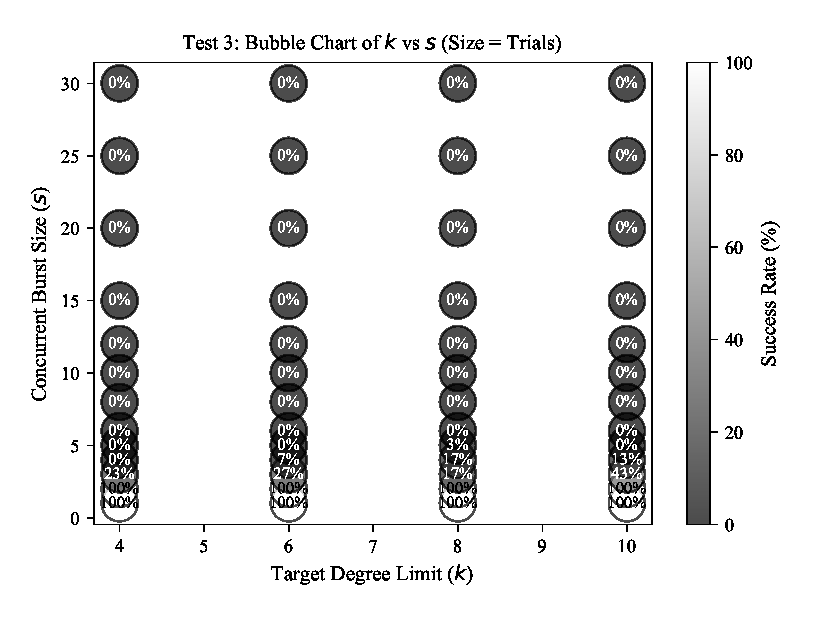
\includegraphics[width=0.49\textwidth]{eval_fig/test3_bubble_k_vs_s.eps}
\caption{Test 3 (Concurrency and Collision Modeling): (a) Convergence success rate under simultaneous burst joins $s \in [1, 30]$ for degrees $k \in \{4, 6, 8, 10\}$; (b) Parameter sweep bubble chart of $k$ versus $s$ (30 trials per configuration, 1,560 total runs).}
\label{fig:test3_results}
\end{figure}

The empirical results in Fig.~\ref{fig:test3_results} illustrate a distinct phase transition:
\begin{enumerate}
    \item \textbf{Low Concurrency ($s \le 2$):} For single arrivals ($s=1$) and pairwise bursts ($s=2$), the success rate remains strictly 100\% across all $k$. In small bursts, the probability that two joining nodes select the same eviction target within the brief vulnerability window $\tau$ remains negligible.
    \item \textbf{Critical Transition ($s = 3, 4$):} At $s = 3$, performance begins to degrade sharply: the success rate drops to 23.3\% for $k=4$, 26.7\% for $k=6$, 16.7\% for $k=8$, and 43.3\% for $k=10$. At $s = 4$, success plummets to 0\% for $k=4$ and 6.7\% for $k=6$.
    \item \textbf{High-Churn Saturation ($s \ge 6$):} For bursts of $s \ge 6$, the unassisted success rate reaches 0\% across all evaluated degrees.
\end{enumerate}

These empirical observations concretely validate the mathematical model presented in Section~5. 
When multiple nodes sample targets concurrently, the localized request arrival rate at an existing peer $A$ scales as $\lambda_A = \lambda \frac{k}{2n}$. 
Because target nodes enforce an immutable degree ceiling $k$, any node receiving multiple concurrent requests ($X \ge 2$) rejects conflicting join plans. 
The rejected nodes remain deficient ($\deg(u) < k$), preventing network convergence. 
These simulation results precisely quantify the vulnerability window $\tau$, demonstrating both the horizontal stability of FINDING NEMO under moderate churn and the theoretical necessity for subsequent self-healing rewiring mechanisms (such as CHUALANH) during massive simultaneous bursts.

\section{Related Works}
\label{sec:related_works}
Decentralized peer-to-peer (P2P) overlay construction and group membership protocols have been investigated across multiple paradigms. We synthesize existing literature across three foundational sub-areas and contrast our findings through empirical evaluation.

\subsubsection{Peer Sampling and Gossip Overlays.}
Unstructured P2P overlays frequently employ randomized epidemic gossip protocols to construct and maintain dynamic membership. A prominent example is CYCLON~\cite{CYCLONInexpensiveMembership}, which uses periodic, pairwise cache shuffling to create connected topologies with low diameter and low clustering coefficients. While CYCLON produces symmetric degree distributions asymptotically, node degrees in epidemic protocols fluctuate stochastically around a target mean with non-zero variance ($\sigma^2 > 0$), rather than satisfying a strict degree bound. In resource-constrained domains, Medley~\cite{yangMedleyMembershipService2022} adapts gossip-based failure detection for wireless IoT ad-hoc environments by introducing distance-biased target selection to reduce multi-hop transmission overhead. However, this optimization intentionally induces non-uniform clustering. In contrast, FINDING NEMO deterministically enforces exact $k$-regularity upon node integration through atomic edge conservation ($\Delta E = k/2$), preventing degree inflation and eliminating structural clustering without requiring iterative shuffling rounds.

\subsubsection{Expander Graphs and Churn Resilience.}
The construction of sparse expander graphs has long been recognized as fundamental for fault-tolerant decentralized communication. Law and Siu~\cite{lawDistributedConstructionRandom2003} proposed a distributed scheme to construct random expander graphs by embedding $d$ edge-disjoint Hamiltonian cycles, using $O(\log n)$ random walks to locate and split existing edges. While theoretically sound, maintaining global Hamiltonian cycles in dynamic environments is fragile: node departures break cycles and necessitate complex stitching mechanisms. Poonpakdee and Di Fatta~\cite{poonpakdeeRobustEfficientMembership2017} introduced EMP+, demonstrating that uncoordinated churn in epidemic protocols inevitably precipitates network partitioning, and employed continuous expansion monitoring to preserve global connectivity. Recently, Gupta and Pandurangan~\cite{guptaFullyDistributedProtocolConstructing2025} formalized the maintenance of bounded-degree expanders under stochastic churn in the presence of full-information Byzantine adversaries, utilizing synchronized random walks. FINDING NEMO departs from these approaches by eliminating rigid cycle dependencies and multi-hop walk overhead; instead, it enforces bounded $k$-regularity via localized, single-hop eviction hand-offs ($O(1)$ operations per target). Furthermore, our structural analysis proves that the probability of topological fragmentation decays exponentially as $P(\text{split}) = p^{2(k+1)^2}$, providing analytical partition resistance that directly resolves the vulnerabilities highlighted by EMP+~\cite{poonpakdeeRobustEfficientMembership2017}.

\subsubsection{Health Checking and Topology Supervision.}
In decentralized failure detection, the SWIM protocol family decouples weakly consistent membership state from health monitoring. Lifeguard~\cite{dadgarLifeguardLocalHealth2017} introduces Local Health Awareness (LHA), dynamically scaling suspicion timeouts and probing periods when local CPU or network queues degrade, thereby suppressing cascading false positives. Medley~\cite{yangMedleyMembershipService2022} similarly addresses failure detection latency under lossy wireless constraints. While Lifeguard and Medley operate along the temporal and protocol dimensions (adjusting detection intervals and probe targets based on local node stress), FINDING NEMO addresses the fundamental topological prerequisite: ensuring that every node is supervised by an exact, uniform number $k$ of independent peers. This invariant prevents under-monitored nodes (which suffer delayed failure detection) as well as over-subscribed nodes (which become message bottlenecks and trigger false-positive alerts).

\subsubsection{Comparative Evaluation and Concurrency Boundaries.}
Our empirical evaluations in Section~\ref{sec:simulation_results} concretely substantiate these theoretical distinctions. Under sequential churn (Test 2), whereas randomized gossip protocols (e.g., CYCLON~\cite{CYCLONInexpensiveMembership}) maintain degree distributions that are only statistically symmetric with persistent variance ($\sigma^2 > 0$) or risk duplicate-induced link deletions under churn (EMP+~\cite{poonpakdeeRobustEfficientMembership2017}), FINDING NEMO deterministically preserves exact $k$-regularity ($\sigma^2 = 0$). Across all evaluated degree limits $k \in \{4, 6, 8, 10\}$ and churn batches up to $g=100$ sequential arrivals, our protocol achieves a 100\% join success rate, demonstrating strict edge conservation without structural degradation. Under concurrent join bursts (Test 3), our experiments isolate the exact vulnerability window ($\tau$) formalized in our Poisson collision model ($\lambda_A = \lambda \frac{k}{2n}$): join operations achieve more than 50\% success for burst sizes $s \le 2$ in an $k + 1$-node overlay, but the performance are drastically improved in a large network. Nevertheless, a rewiring mechanism (such as CHUALANH) is necessary to overcome this challenge.

\section{Concluding Remarks and Future Work}
In this paper, we introduced FINDING NEMO, a highly scalable, decentralized join-and-evict protocol designed to construct and maintain random regular overlays. 
By mathematically isolating the exact rules of node integration, we demonstrated that localized eviction and rewiring is mandatory to preserve bounded-degree properties. 
Furthermore, by formalizing the concurrent bootstrap race through a Poisson arrival model, we clearly defined the protocol's upper limits under massive simultaneous churn. 
Future work will focus on integrating a decentralized self-healing mechanism (such as CHUALANH) to automatically repair the deficient nodes caused by these concurrent broadcast collisions, as well as evaluating performance under heterogeneous latency distributions. 

% \section{First Section: This is used for example only}
% \subsection{A Subsection Sample}
% Please note that the first paragraph of a section or subsection is
% not indented. The first paragraph that follows a table, figure,
% equation etc. does not need an indent, either.

% Subsequent paragraphs, however, are indented.

% \subsubsection{Sample Heading (Third Level)} Only two levels of
% headings should be numbered. Lower level headings remain unnumbered;
% they are formatted as run-in headings.

% \paragraph{Sample Heading (Fourth Level)}
% The contribution should contain no more than four levels of
% headings. Table~\ref{tab1} gives a summary of all heading levels.

% \begin{table}
% \caption{Table captions should be placed above the
% tables.}\label{tab1}
% \begin{tabular}{|l|l|l|}
% \hline
% Heading level &  Example & Font size and style\\
% \hline
% Title (centered) &  {\Large\bfseries Lecture Notes} & 14 point, bold\\
% 1st-level heading &  {\large\bfseries 1 Introduction} & 12 point, bold\\
% 2nd-level heading & {\bfseries 2.1 Printing Area} & 10 point, bold\\
% 3rd-level heading & {\bfseries Run-in Heading in Bold.} Text follows & 10 point, bold\\
% 4th-level heading & {\itshape Lowest Level Heading.} Text follows & 10 point, italic\\
% \hline
% \end{tabular}
% \end{table}


% \noindent Displayed equations are centered and set on a separate
% line.
% \begin{equation}
% x + y = z
% \end{equation}
% Please try to avoid rasterized images for line-art diagrams and
% schemas. Whenever possible, use vector graphics instead (see
% Fig.~\ref{fig1}).

% \begin{figure}
% 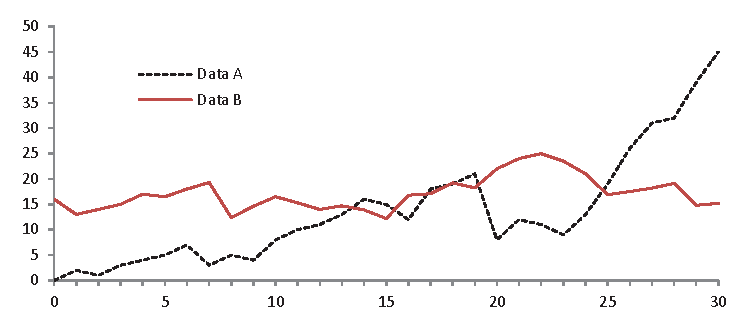
\includegraphics[width=\textwidth]{fig1.eps}
% \caption{A figure caption is always placed below the illustration.
% Please note that short captions are centered, while long ones are
% justified by the macro package automatically.} \label{fig1}
% \end{figure}

% \begin{theorem}
% This is a sample theorem. The run-in heading is set in bold, while
% the following text appears in italics. Definitions, lemmas,
% propositions, and corollaries are styled the same way.
% \end{theorem}
% %
% % the environments 'definition', 'lemma', 'proposition', 'corollary',
% % 'remark', and 'example' are defined in the LLNCS documentclass as well.
% %
% \begin{proof}
% Proofs, examples, and remarks have the initial word in italics,
% while the following text appears in normal font.
% \end{proof}
% For citations of references, we prefer the use of square brackets
% and consecutive numbers. Citations using labels or the author/year
% convention are also acceptable. The following bibliography provides
% a sample reference list with entries for journal
% articles~\cite{ref_article1}, an LNCS chapter~\cite{ref_lncs1}, a
% book~\cite{ref_book1}, proceedings without editors~\cite{ref_proc1},
% and a homepage~\cite{ref_url1}. Multiple citations are grouped
% \cite{ref_article1,ref_lncs1,ref_book1},
% \cite{ref_article1,ref_book1,ref_proc1,ref_url1}.

% \begin{credits}
% \subsubsection{\ackname} A bold run-in heading in small font size at the end of the paper is
% used for general acknowledgments, for example: This study was funded
% by X (grant number Y).

% \subsubsection{\discintname}
% It is now necessary to declare any competing interests or to specifically
% state that the authors have no competing interests. Please place the
% statement with a bold run-in heading in small font size beneath the
% (optional) acknowledgments\footnote{If EquinOCS, our proceedings submission
% system, is used, then the disclaimer can be provided directly in the system.},
% for example: The authors have no competing interests to declare that are
% relevant to the content of this article. Or: Author A has received research
% grants from Company W. Author B has received a speaker honorarium from
% Company X and owns stock in Company Y. Author C is a member of committee Z.
% \end{credits}
% %
% % ---- Bibliography ----
% %
% % BibTeX users should specify bibliography style 'splncs04'.
% % References will then be sorted and formatted in the correct style.
% %
\bibliographystyle{splncs04}
\bibliography{findingnemo}
% %
% \begin{thebibliography}{8}
% \bibitem{ref_article1}
% Author, F.: Article title. Journal \textbf{2}(5), 99--110 (2016)

% \bibitem{ref_lncs1}
% Author, F., Author, S.: Title of a proceedings paper. In: Editor,
% F., Editor, S. (eds.) CONFERENCE 2016, LNCS, vol. 9999, pp. 1--13.
% Springer, Heidelberg (2016). \doi{10.10007/1234567890}

% \bibitem{ref_book1}
% Author, F., Author, S., Author, T.: Book title. 2nd edn. Publisher,
% Location (1999)

% \bibitem{ref_proc1}
% Author, A.-B.: Contribution title. In: 9th International Proceedings
% on Proceedings, pp. 1--2. Publisher, Location (2010)

% \bibitem{ref_url1}
% LNCS Homepage, \url{http://www.springer.com/lncs}, last accessed 2023/10/25
% \end{thebibliography}
% \begin{credits}
% \subsubsection{\ackname} 
% This study was conducted as part of distributed systems research at the Vietnamese-German University.

% \subsubsection{\discintname}
% The authors have no competing interests to declare that are relevant to the content of this article.
% \end{credits}

% \begin{thebibliography}{8}
% \bibitem{ref_article1}
% Author, F.: Article title. Journal \textbf{2}(5), 99--110 (2016)
% % Placeholder for actual references
% \end{thebibliography}
\end{document}
